\documentclass[10pt,a4paper]{article}
\usepackage[latin1]{inputenc}
\usepackage{amsmath}
\usepackage{amsfonts}
\usepackage{amssymb}
\usepackage{makeidx}
\usepackage{graphicx}
\usepackage{caption}
\usepackage{subcaption}
\usepackage{float}
\usepackage{wrapfig}
\usepackage[left=1.00in, right=1.00in, top=1.00in, bottom=1.00in]{geometry}
\usepackage{tikz}
\usetikzlibrary{matrix,positioning,calc,intersections,arrows,fadings}
\begin{document}
\title{TI Competition}
\author{Adam Leach, Edward Sainsbury, Kaiwen Lin, Oliver Groeling, Usmaan Javed}
\maketitle
\tableofcontents
\section{CAN Protocol}
[BRIEF DESCRIPTION OF CAN AND WHY ITS BEING USED]

[PRETTY SCHEMATIC/BLOCK DIAGRAM TO DO WITH CAN]

[EXPLANATION OF PRETTY PICTURE AND VERY BRIEF SUMMARY]
\section{Driver Controls}

The driver will need to be able to directly control several electronic systems while in a driving position. These systems include the Electric Vehicles directional indicators, the speed of the vehicle, the direction the vehicle is travelling in as well as being able to place the car in its safe state. While in its safe state the batteries must be isolated from the rest of the vehicle. The driver will also have to be able to exit the safe state while in the drivers seat. 

Apart from being able to control systems the driver must also be relayed important information such as the speed of the vehicle, the state of charge of the batteries as well as being alerted of any faults which develop.

\subsection{Directional Indicators}

To comply with regulations the vehicle must have indicators which alert other road users of the drivers intentions. [REWORD A BIT CLUNKY] The indicators must pulse on and off at 90 pulses per minute when the indicators are active. 

\begin{figure}[H]
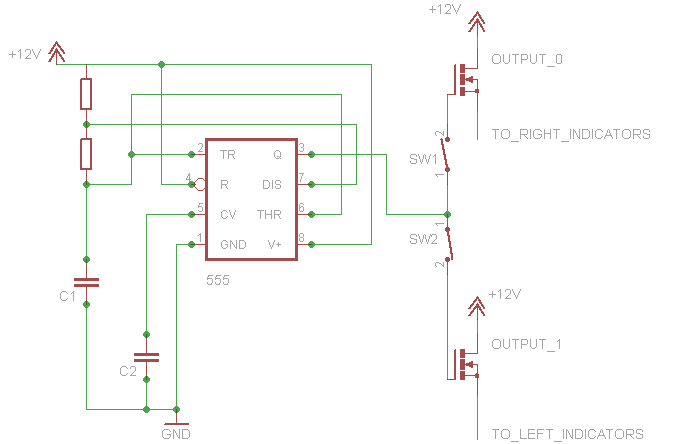
\includegraphics[width=\columnwidth]{555Circuit}%
\caption{Wiring Diagram of the Indicator Drivers}
\label{Fig:IndicatorWiring}
\end{figure}

As shown in Figure \ref{Fig:IndicatorWiring} a 555 timer is used to control a 12V bus which powers the LEDs. Due to the curvature on the front of the vehicle the front indicators are flexible LED strips which we can mould to the vehicles shape. However, the rear indicators use a specially designed LED strip with a constant current driver. [NOT SURE WHETHER TO GO INTO MORE DETAIL OF THE CONST. CURRENT]

\subsection{Brake Lights}

Rear brake lights must be fitted to the vehicle which activate automatically when the driver activates the brakes. In order to detect when the driver applies the brakes a micro switch is fitted to the brake pedal and hand brake lever. The switches are wired in parallel and control the power going to the brake light drivers. 

\begin{figure}[H]
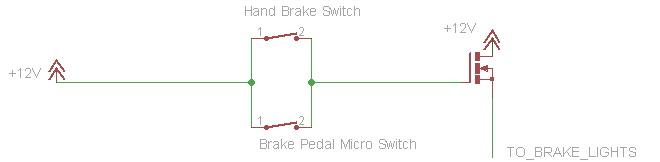
\includegraphics[width=\columnwidth]{BrakeLightControl.png}%
\caption{Brake Light Control Schematic}
\label{Fig:BrakeLightsWiring}
\end{figure}

\subsection{Controlling the Motor}
In order to set the speed of the vehicle the motor controller needs to be sent messages with a target speed for the motor. The motor controller uses this information to control the amount of power fed into the motor in order to control its speed. The messages are sent via the CAN bus of the vehicle allowing for any device attached to the CAN bus to have access to information such as speed and motor power consumption. 

As the driver would likely be travelling at roughly the same speed for the entirety of their three hour sessions it was decided that a cruise control system would be most suitable. Where the driver holds down a dead man switch and controls the speed using a potentiometer located near the driver.

The device which takes take of all the driver inputs is known as the main controller. The main controller reads the state of the accelerator pedal which acts as a dead man switch. If the accelerator is pressed the main controller then reads the value of the speed control which acts as an analogue input to the main controller. After encoding the analogue value it is sent over the CAN bus to the motor controller. A third input is attached to the main controller which controls whether the motor will go forwards, backwards or act as a brake. This tristate switch when in the forward state will cause the main controller to behave as previously described. When in the brake state it will cause the main controller to only send the motor controller a command which tells it to keep the motor stationary. This command will be sent until the switch is placed into another state. Finally, if the switch is placed into the reverse position the main controller will activate the rear view camera as well as altering the speed command that is sent to the motor controller such that it will cause the motor to rotate backwards.

\begin{figure}[H]
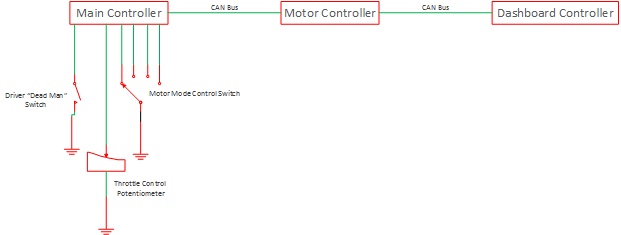
\includegraphics[width=\columnwidth]{MotorControlDiagram.png}%
\caption{Motor Communication Diagram}
\label{Fig:MotorControl}
\end{figure}

\subsection{Vehicle Safe State}
The electric vehicles safe state causes the only conductors that leave the battery box to be galvanically isolated from the batteries. It also causes the solar array to be disconnected from the electrical systems. 

In order to enter this state a normally closed button wired in series to the relay control mechanism is pressed. This will interrupt power to the relay control which will cause the relays to return to their normally open position.

\begin{figure}[H]
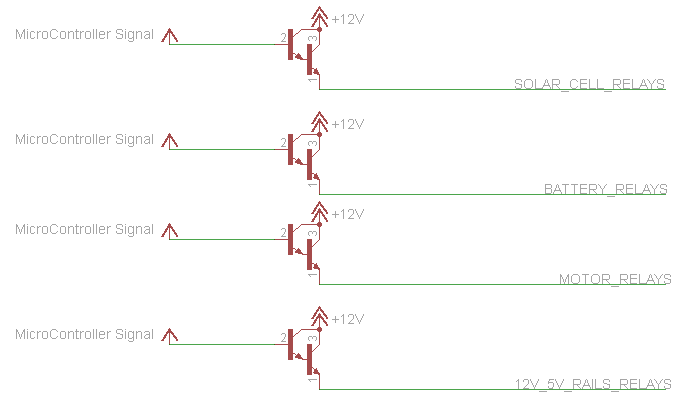
\includegraphics[width=\columnwidth]{RelayControl.png}%
\caption{Relay Control Mechanism}
\label{Fig:RelayControl}
\end{figure}

In order to close a relay a 5V signal must be sent from a micro controller which feeds into a Darlington Transistor which controls a 12V signal which is then wired up to the coils of normally open relays. So when both a 5V signal and a 12V rail is attached the relays will close. TO enter the safe state the 12V or the 5V rail must be deactivated which is done by controlling a relay wired in series to the rails.

Only a few devices can control the 5V signal which can be used to disconnect individual relays. These devices are the main controller and a second controller which operates many of the safety systems. The second controller is interfaced with temperature sensors attached to each cell on the batteries through a one wire bus so it is able to isolate parts of the vehicle automatically if for instance a battery gets too hot it can place the vehicle to the safe state. Or if a part of the array is malfunctioning it can isolate that part of the array as well as alerting the driver to the malfunction.

Once in the safe state the problem of exiting the safe state arises. Both the 12V and 5V rail have to be enabled to exit the safe state, as opposed to entering which only required disabling one of the rails. Furthermore, the driver must be able to do this from within the drivers seat meaning the system must be galvanically isolated. In order to do this a seperate isolated DCDC converter is used. This supply can control the relays necessary to exit the safe state and so by wiring up a mechanical switch the driver can easily exit the safe state

\begin{figure}[H]
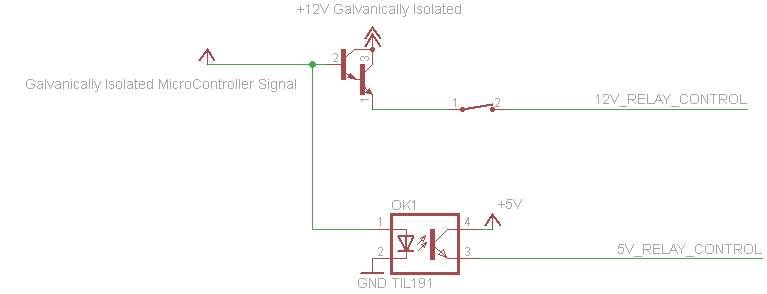
\includegraphics[width=\columnwidth]{SafeStateIsolated.png}%
\caption{Galvanically Isolated Relay Control}
\label{Fig:IsolatedControl}
\end{figure}


\section{Sensors}
The sensors attached to the vehicle will allow the team to better analyse and predict the vehicles behaviour as well as offering forewarnings for future issues sensor data may also be used to further refine future designs of key components. Sensors will interface with a micro controller which will do some pre processing of the data before sending the data onto the CAN bus. It will then be logged on the data logger and sent via the telemetry system to the team. Some sensor data will also be displayed directly to the driver. 

\subsection{Temperature}
A Dallas one wire bus is used to interface temperature sensors from around the car. The micro controller will then monitor for any abnormal behaviour to alert the driver of as well as sending all the temperature data to the data logger. [INCLUDE SCHEMATIC]

\subsection{Light Sensors}
Photodiodes attached to the photo voltaic array will allow the monitoring of individual solar panels. The data from the the photo diodes coupled with the current monitors attached to the output of the MPPTs allow for the performance of the array to be monitored as well as allowing the detection of oncoming failures before they are able to become catastrophic. The data will also allow improvements to be made on the design of future MPPTs and solar arrays. [SCHEMATIC] 

\subsection{GPS}
The Beagle Bone black is fitted with a GPS module which allows for an accurate time source within the vehicle as well as a secondary speed measurement. [NEED MORE INFO HERE]

\subsection{Current Monitoring}
Detecting the current produced from the solar array as well as the current the batteries output allows key data on power consumption and generation to be gathered. In order to measure the current hall effect based sensors are used within the vehicle. [MORE DETAIL NEEDED]

\subsection{Battery Voltage}

The battery voltage is proportional to charge and so by monitoring the voltage a rough estimation on the state of charge can be found. It also allows for the health of the batteries to be monitored. The motor controller has a built in voltage transducer which measures the input voltage and even transmit this information over the CAN bus. This is the system currently in use which allows for a battery monitoring algorithm to be developed in the future.

\subsection{Strain Gauges}
In order to improve future designs of structural components within the vehicle strain gauges are fitted on to them so the performance of structural components can be monitored and analysed. [NEED MORE DETAIL]


\section{Telemetry}
A crucial part of the project is the system that handles the large volume of data the CAN bus receives. This system must be able to efficiently store data, facilitate the sending of operation critical messages and provide meaningful feedback to the client.Telemetry is required to effectively analyze the system with both quantitative and qualitative data. This data will allow engineers to monitor the status of the system and make important decisions which could affect its performance. The proposed system can be broken down as follows: a CAN bus interface, a data logger, an SQL database, a graphical user interface to allow engineers to remotely access and send data.
\begin{wrapfigure}{r}{0.5\textwidth}
         \centering
         \begin{subfigure}[b]{0.6\textwidth}
              %   \includegraphics[width=\textwidth]{canusb}
                 \caption{A CANUSB adaptor}
                 \label{fig:CANUSB adaptor}
         \end{subfigure}

         \begin{subfigure}[b]{0.4\textwidth}
              %   \includegraphics[width=\textwidth]{beaglebone}
                 \caption{A Beagle Bone Black}
                 \label{fig:Beable Bone Black}
         \end{subfigure}

         \begin{subfigure}[b]{0.5\textwidth}
              %   \includegraphics[width=\textwidth]{server}
                 \caption{A Server}
                 \label{fig:Sever}
         \end{subfigure}
         \caption{Components of the telemetry system}\label{fig:telemetry}
\end{wrapfigure}
The first component of the telemetry system is the interface between the data logger and the CAN bus. This connection is made with an adapter which connects directly in between the CANBUS and the data logger which is then controlled by the data handling software on the data logger.

The data is filtered by node and data type and is then saved to an SQL server running on the data logger. It is critically important that the data logger program can handle errors and consistently. If the program were to crash or incorrectly filter the data, the system could give incorrect data to the engineers leading to erroneous decisions or could completely stop working.

Once the data has been saved to the SQL server, the engineers can access or send data remotely over a tcp connection via a separate program on their computer.

This is clearly a very powerful system allowing telemetry data to be sent and received from, theoretically,  anywhere in the world. If for example the nodes where in fact not just sensors but active components, it would be conceivable to drive the car from anywhere with an internet connection, thousands of miles away from the car itself.

\section{Voltage Rails}
In order to create 12V and 5V rails from the 48V unregulated batteries the LM2576HV was used as a buck converter to regulate and step down the voltage. However, the 3A maximum output current would not be enough to power all the systems within the vehicle. To resolve this issue several modules where used and daisy chained together in order to provide rails which can provide a sufficient amount of power for all the systems. [USES TI CHIP SO THOUGHT SHOULD ADD THIS. NOT SURE IF I SHOULD INCLUDE A SCHEMATIC] 
\end{document}
